\section{Preliminaries}
\label{sec:prelim}

\paragraph{Craig interpolation~\cite{MR0104564}.}
We consider Craig interplants for quantifier-free first-order formulas. Given two formulas $A$ and $B$, such that $A ∧ B$ is unsatisfiable, an interpolant $I$ is a formula satisfying:
\begin{itemize}
\item $A ⇒ I$;
\item $B ∧ I ⇒ ⊥$;
\item $fv(I) ⊆ fv(A) ∩ fv(B)$ where $fv(\cdot)$ returns the free variables in a formula.
\end{itemize}
\begin{notation}
We use the meta-level symbol $\Rightarrow$ as a shorthand for logical implications in texts. In the proof rules that we will introduce shortly, $\vdash$ is used as the formal symbol with the standard interpretation as logical derivations. 
\end{notation}

\paragraph{Delta-Complete Decision Procedures.}

We consider first-order formulas interpreted over the real numbers. Our special focus is formulas that can contain arbitrary nonlinear functions that are {\em Type 2 computable}~\cite{CAbook,vasco}. Intuitively, Type 2 computability corresponds to {\em numerical computability}. For our purpose, it is enough to note that this set of functions consist of all common elementary functions, as well as solutions of Lipschitz-continuous ordinary differential equations. 

Interval Constraint Propagation (ICP)~\cite{handbookICP} finds
solutions of real constraints using the \emph{branch-and-prune} method, combining
interval arithmetic and constraint propagation. The idea is to use interval
extensions of functions to \emph{prune} out sets of points that are not in the
solution set and \emph{branch} on intervals when
such pruning can not be done, recursively until a small enough box
that may contain a solution is found or inconsistency is observed.
A high-level description of the decision version of ICP is given in Algorithm~\ref{icpalgo}~\cite{handbookICP,DBLP:conf/cade/GaoAC12}.
The boxes, or interval domains, are written as $\vec D$ and $c_i$ denotes the $i$th constraint.
\begin{algorithm}\label{algo1}
\caption{ICP($c_1,...,c_m, \vec D = D_1\times\cdots\times D_n, \delta$)}\label{icpalgo}
\begin{algorithmic}[1]
\Statex
    \State $S \gets \vec D$
    \While{$S \neq \emptyset$}
        \State $\vec D \gets S.\mathrm{pop}()$
        \While{$\exists 1 \leq i \leq m, \vec D \neq_{\delta} \mathrm{Prune}(\vec D,c_i)$}
        \State $\vec D \gets \mathrm{Prune}(\vec D, c_i)$
        \EndWhile
        \If{$\vec D \neq \emptyset$}
            \If{$\exists 1\leq i\leq m, |\vec D|\geq \varepsilon$} \Comment{$\varepsilon$ is some computable factor of $\delta$}
                \State $\{\vec D_1,\vec D_2\} \gets \mathrm{Branch}(\vec D, i)$
                \State $S.\mathrm{push}(\vec D_1)$
                \State $S.\mathrm{push}(\vec D_2)$
            \Else
                \State \Return {\sf sat}
            \EndIf
        \EndIf
    \EndWhile
    \State \Return {\sf unsat}
\end{algorithmic}
\end{algorithm}

%   \begin{example}
%   Consider a constraint $c(x,y) : y=x \wedge y = x^2$, and $x\in [1.5,2]$ and
%   $y\in [1,2]$ are the initial interval assignment. We use the abstract-DPLL style notation $\vec x\in \vec D||c$ to denote the pair of the sequence of interval assignments. (For more details, see~\cite{DBLP:conf/synasc/GaoKC13}.) A run of the ICP algorithm on this problem is as follows:
%   \begin{eqnarray*}
%   & &x\in [1.5,2], y\in [1,2]\parallel c \\
%   &\stackrel{branch}{\Longrightarrow}& x\in [1.5,2],
%   y\in [1,2], (x\in [1.7, 2])^d\parallel c\\
%   & &\mbox{  (branching on the x variable, looking only at the part $x\in[1.7,2]$)}\\
%   &\stackrel{backtrack}{\Longrightarrow}& x\in [1.5,2], y\in [1,2], x\in [1.5, 1.7]\parallel c\\
%   & &\mbox{  (backtracking, since $\forall\vec a\in [1.7,2]\times [1,2]$,
%   $c(\vec a)$ is false,}\\
%   & & \hspace{4cm} \mbox{and $[1.5,2]\subseteq[1.5,1.7]\cup [1.5, 2]$ for
%   $x$)}\\
%   &\stackrel{prune}{\Longrightarrow}& x\in [1.5,2], y\in [1,2], x\in [1.5, 1.7], x\in
%   [1.5, 1.6]\parallel c\\
%   & & \mbox{  (pruning, since $\forall \vec a\in[1.6,1.7]\times [1, 2]$, $c(\vec
%   a)$ is false)}\\
%   &\stackrel{prune}{\Longrightarrow}& x\in [1.5,2], y\in [1,2], x\in [1.5, 1.7],x\in [1.5, 1.6], x\in \emptyset\parallel c\\
%   & & \mbox{  (pruning, since $\forall \vec a\in[1.5,1.6]\times [1, 2]$, $c(\vec
%   a)$
%   is false)}\\
%   &\stackrel{fail}{\Longrightarrow}& \emptyset||c\ \mbox{ (since
%   $\forall \vec a\in \emptyset \times [1, 2], c(\vec a)$ is false.)}
%   \end{eqnarray*}
%   In the last step, the algorithm concludes that there is a conflict between the assignment sequence and the constraint, because $x\in \emptyset$ has been derived. 
%   \end{example}

\paragraph{Proofs from constraint propagation.}

A detailed description of proof extraction from $\delta$-decision procedure is available in~\cite{DBLP:conf/synasc/GaoKC14}.
Here, we use a simplified version. Intuitively, the proof of unsatisfiability recursively divides the solution space to small pieces, until it can prove (mostly using interval arithmetic) that every small piece of the domain contains no solution of the original system. Note that in such a proof, the difference between pruning and branching operations become blurred for the following reason. Pruning operations show that one part of the domain can be discarded because no solution can exist there. Branching operations split the domain along one variable, and generates two sub-problems. From a proof perspective, the difference between the two kinds of operations is simply whether the emptiness in one part of domain follows from a simple properties of the functions (theory lemma), or requires further derivations. Indeed, as is shown in~\cite{DBLP:conf/synasc/GaoKC14}, the simple proof system in Figure~\ref{fig:rules} is enough for establishing all theorems that can be obtained by $\delta$-decision procedures. The rules can be explained as follows. 
\begin{itemize}
\item The \splt rules divides the solution space into two disjoint subspaces.
\item The theory lemmas (\thLem) are the leaves of the proof. They are used when the solver managed to prove the absence of solution in a given subspace.
\item The \weaken rule extracts those conjunct out of the main formula.
\end{itemize}
We see that each step of the proof has a set of variables $\vec x$ with a domain $\vec D$ and $F$ is a formula. We use of vectors in the formulas, writing $\vec x ∈ \vec D$ to denote $\bigwedge_i x_i ∈ D_i$. The domains are intervals, i.e., each $D_i$ has the form $[l_i,u_i]$ where $l_i$,$u_i$ are the lower and upper bounds for $x_i$. Since we are looking at unsatisfiability proofs, each node implies $⊥$. The root of the proof is has formula $A ∧ B$ and $D$ covers the entire domain, the inner nodes are \splt, and the proof's leaves are theory lemmas directly followed by weakening. To avoid duplication we do not give a seperate example here, since the full example in Figure~\ref{fig:proof} shows the structure of some proof trees obtained from such rules. 

\begin{figure}
\centering
\begin{mathpar}
\inferrule{ {} }{
  \vec x ∈ \vec D ∧ c \entails ⊥
}{(\thLem)}\\

\inferrule{
  C := c ∧ \bigwedge_k C_k \\
  \vec x ∈ \vec D ∧ c \entails ⊥
}{
  \vec x ∈ \vec D ∧ C \entails ⊥
}{(\weaken)}\\

\inferrule{
  x_i ∈ [l_i, p] ∧ \bigwedge_{j ≠ i} x_j ∈ D_j ∧ C \entails ⊥ \\
  x_i ∈ [p, u_i] ∧ \bigwedge_{j ≠ i} x_j ∈ D_j ∧ C \entails ⊥
}{
  x_i\in [l_i, u_i] \wedge \bigwedge_{j\neq i} x_j∈ D_j ∧ C \entails ⊥
}{(\splt)}
\end{mathpar}
\caption{Proof rules for the ICP algorithm. We use the standard notations for sequent calulus. Also, when we write an interval $[a,b]$, we always assume that it is a well-defined real interval satisfying $a\leq b$. 
}
\label{fig:rules}
\end{figure}

Algorithm~\ref{icpalgo} generates proof during the \emph{branching} and \emph{pruning} operations.
Branching directly corresponds to the $\splt$ rule.
Pruning, on the other hand, is a combination of the three rules.
Let us look at $\vec D' = \text{Pruning}(\vec D, c_i)$.
The constraint $c_i$ is selected with the \weaken.
For each $D'_i=[l',u']$ which is strictly smaller than $D_i=[l,u]$, the \splt and \thLem rules are applied.
If $u'<u$ then we split on $u'$ and a lemma shows that the interval $[u,u']$ has no solution.
The same is done for the lower bounds $l'$,$l$.
Figure~\ref{fig:prune} shows a pruning step and the corresponding proof.

\begin{figure}
\centering
\begin{tikzpicture}
\node (n0) at (-1.2, 0.1) {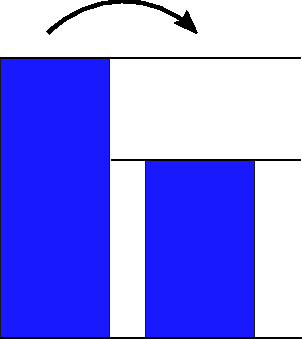
\includegraphics[scale=0.4]{img/pruning.pdf}};
\node (n1) at ( 0.0, 0.85) {$u$};
\node (n2) at ( 0.05, 0.2) {$u'$};
\node (n3) at ( 0.0,-1.0) {$l$};
\node (n4) at (-1.0, 1.5) {pruning by $c_i$};
\node (n5) at (0.8, -0.2) {\large \ldots};
\node (n6) at (6.0, 0.0) {\begin{minipage}{0.7\textwidth}
{\small
\begin{mathpar}
\inferrule{
    \vdots\\
    \inferrule{
        \inferrule{ {} }{ x ∈ [u',u] ∧ c_i \entails ⊥ }{(\thLem)}
    }{
        x ∈ [u',u] ∧ c_i ∧ \bigwedge_{k≠i} c_k \entails ⊥ 
    }{(\weaken)} \\
}{
    x ∈ [l,u] ∧ \bigwedge_k c_k \entails ⊥
}{(\splt)}
\end{mathpar}
}
\end{minipage}
};
\end{tikzpicture}
\caption{
    Pruning operation and the corresponding proof.
    The pruning shrinks the domain of $x$ from $[l,u]$ to $[l,u']$.
    The corresponding proof starts with a \splt around $u'$.
    The interval $[u',u]$ is proved empty using a \thLem and \weaken step.
    The remaining $[l,u']$ interval is shown empty by further operations.
}
\label{fig:prune}
\end{figure}
